\documentclass[12pt]{article}
\usepackage[paper=letterpaper,margin=2cm]{geometry}
\usepackage{amsmath}
\usepackage{amssymb}
\usepackage{amsfonts}
\usepackage{newtxtext, newtxmath}
\usepackage{enumitem}
\usepackage{titling}
\usepackage[colorlinks=true]{hyperref}
\usepackage{graphicx}
\usepackage{float}
\usepackage{listings}
\usepackage{xcolor}
\usepackage{color}
\usepackage{caption}
\usepackage{subfigure}
\usepackage{float}

\usepackage{booktabs}
\usepackage{multirow}

\definecolor{dkgreen}{rgb}{0,0.6,0}
\definecolor{gray}{rgb}{0.5,0.5,0.5}
\definecolor{mauve}{rgb}{0.58,0,0.82}
\lstset{ %
        language=Java,                
  basicstyle=\footnotesize,     
  numbers=left,               
  numberstyle=\tiny\color{gray},
  stepnumber=1,                                       
  numbersep=5pt,                 
  backgroundcolor=\color{white},  
  showspaces=false,             
  showstringspaces=false,         
  showtabs=false,                 
  frame=single,                   
  rulecolor=\color{black},       
  tabsize=4,                   
  captionpos=b,        
  breaklines=true,             
  breakatwhitespace=false,       
  title=\lstname,                                                  
  keywordstyle=\color{blue},          
  commentstyle=\color{dkgreen},    
  stringstyle=\color{mauve},       
  escapeinside={\%*}{*},        
  morekeywords={*,...}
} 

\setlength{\droptitle}{-6em}

% Enter the specific assignment number and topic of that assignment below, and replace "Your Name" with your actual name.
\title{Assignment 3: Comp 6771 Image Processing}
\author{Yunqi Xu 40130514}
\date{\today}



\begin{document}
% \maketitle

\begin{titlepage}
  \rule{\textwidth}{1pt}   % The top horizontal rule
    \vspace{0.2\textheight}  % Whitespace between top horizontal rule and title

    %------------------------------------------------------------
    %    Title
    %------------------------------------------------------------

    {\Huge COMP 6771 Image Processing: Assignment 2}

    \vspace{0.025\textheight}   % Whitespace between the title and short horizontal rule

    \rule{0.83\textwidth}{0.4pt}  % The short horizontal rule under title

    \vspace{0.1\textheight}  % Whitespace between the short horizontal rule and author

    %------------------------------------------------------------
    %    Author
    %------------------------------------------------------------

    {\Large Student name: \textsc{Yunqi Xu}}
    \vfill
    {\Large Student id: 40130514}
    \vfill  % Whitespace between author and date

    {\large \today}
    \vspace{0.1\textheight}  % Whitespace between date and bottom horizontal rule

    %------------------------------------------------------------
    %    Bottom rules
    %------------------------------------------------------------

    \rule{\textwidth}{1pt}  % The bottom horizontal rule
\end{titlepage}

\section{Review}
\subsection{Review of Bilateral Filter}
% overall summary of bilateral filter
Bilateral Filter is one of the most important filter method which presented by Tomasi in 1998. 
The bilateral filter smoothing image and preserve edges information at the meanwhile.

% review of the bilateral filter method
The main method that the bilateral filter utilized are two Gaussian filters. 
One is calcualted based on the Geometric closeness. 
Another is calculated based on their photometric similarity
% achievement



\subsection{Review of another paper}
% In this section, first introduce another method that provided by other paper, and then compared with the Bilateral filter


\section{Re-impleement of Bilateral Filter}
In this section, we will firstly present the result of our re-implement method, and then compared the bilater filter with other baseline algorithm in terms of other low pass filters that usually blur the image but also blur edges


\subsection{Result of the Re-implement algorithm}
In this section, we will use the images in the paper[cite here] to show our result that has successfully achieve the main goal which introduced by the paper.

Firstly, we present our result compared with the result indicated in the paper, with the same inputted parameters and the same pattern.

\begin{figure}[H]
  \centering
  \subfigure[$\sigma_d=1, \sigma_r=10$]{
  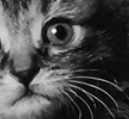
\includegraphics[width=3.5cm]{output_image/cat_part_ds1_rs10.png}
  % \caption{fig1}
  }
  \quad
  \subfigure[$\sigma_d=1, \sigma_r=30$]{
  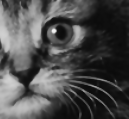
\includegraphics[width=3.5cm]{output_image/cat_part_ds1_rs30.png}
  }
  \quad
  \subfigure[$\sigma_d=1, \sigma_r=100$]{
  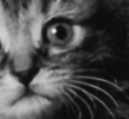
\includegraphics[width=3.5cm]{output_image/cat_part_ds1_rs100.png}
  }
  \quad
  \subfigure[$\sigma_d=1, \sigma_r=300$]{
  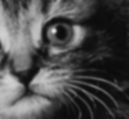
\includegraphics[width=3.5cm]{output_image/cat_part_ds1_rs300.png}
  }

  \subfigure[$\sigma_d=3, \sigma_r=10$]{
  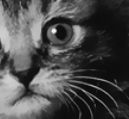
\includegraphics[width=3.5cm]{output_image/cat_part_ds3_rs10.png}
  % \caption{fig1}
  }
  \quad
  \subfigure[$\sigma_d=3, \sigma_r=30$]{
  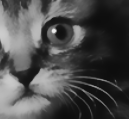
\includegraphics[width=3.5cm]{output_image/cat_part_ds3_rs30.png}
  }
  \quad
  \subfigure[$\sigma_d=3, \sigma_r=100$]{
  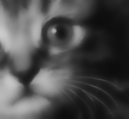
\includegraphics[width=3.5cm]{output_image/cat_part_ds3_rs100.png}
  }
  \quad
  \subfigure[$\sigma_d=3, \sigma_r=300$]{
  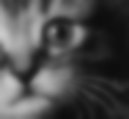
\includegraphics[width=3.5cm]{output_image/cat_part_ds3_rs300.png}
  }

  \subfigure[$\sigma_d=10, \sigma_r=10$]{
  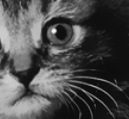
\includegraphics[width=3.5cm]{output_image/cat_part_ds10_rs10.png}
  % \caption{fig1}
  }
  \quad
  \subfigure[$\sigma_d=10, \sigma_r=30$]{
  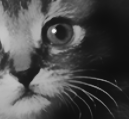
\includegraphics[width=3.5cm]{output_image/cat_part_ds10_rs30.png}
  }
  \quad
  \subfigure[$\sigma_d=10, \sigma_r=100$]{
  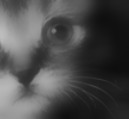
\includegraphics[width=3.5cm]{output_image/cat_part_ds10_rs100.png}
  }
  \quad
  \subfigure[$\sigma_d=10, \sigma_r=300$]{
  
\includegraphics[width=3.5cm]{output_image/cat_part_ds10_rs300.png}
  }
  \caption{A detail figure with bilateral filters with various range and domain parameter values by implement code}
  \label{im_cateye}
  \end{figure}

The Fig.~\ref{im_cateye} presents the result of out implement. In this experiments, we use $kernel\_size = 25$ and other parameters are totally the same as the paper, and we got the same trend of the blur as the paper get.

\begin{figure}[H]
  \centering
  \subfigure[$\sigma_d=1, \sigma_r=10$]{
  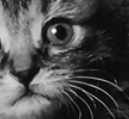
\includegraphics[width=3.5cm]{output_image_python/cat_part_ds1_rs10.png}
  % \caption{fig1}
  }
  \quad
  \subfigure[$\sigma_d=1, \sigma_r=30$]{
  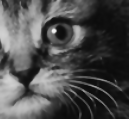
\includegraphics[width=3.5cm]{output_image_python/cat_part_ds1_rs30.png}
  }
  \quad
  \subfigure[$\sigma_d=1, \sigma_r=100$]{
  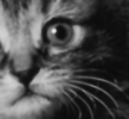
\includegraphics[width=3.5cm]{output_image_python/cat_part_ds1_rs100.png}
  }
  \quad
  \subfigure[$\sigma_d=1, \sigma_r=300$]{
  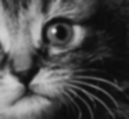
\includegraphics[width=3.5cm]{output_image_python/cat_part_ds1_rs300.png}
  }

  \subfigure[$\sigma_d=3, \sigma_r=10$]{
  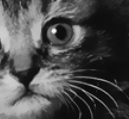
\includegraphics[width=3.5cm]{output_image_python/cat_part_ds3_rs10.png}
  % \caption{fig1}
  }
  \quad
  \subfigure[$\sigma_d=3, \sigma_r=30$]{
  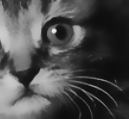
\includegraphics[width=3.5cm]{output_image_python/cat_part_ds3_rs30.png}
  }
  \quad
  \subfigure[$\sigma_d=3, \sigma_r=100$]{
  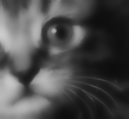
\includegraphics[width=3.5cm]{output_image_python/cat_part_ds3_rs100.png}
  }
  \quad
  \subfigure[$\sigma_d=3, \sigma_r=300$]{
  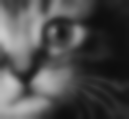
\includegraphics[width=3.5cm]{output_image_python/cat_part_ds3_rs300.png}
  }

  \subfigure[$\sigma_d=10, \sigma_r=10$]{
  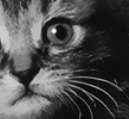
\includegraphics[width=3.5cm]{output_image_python/cat_part_ds10_rs10.png}
  % \caption{fig1}
  }
  \quad
  \subfigure[$\sigma_d=10, \sigma_r=30$]{
  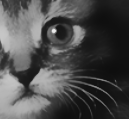
\includegraphics[width=3.5cm]{output_image_python/cat_part_ds10_rs30.png}
  }
  \quad
  \subfigure[$\sigma_d=10, \sigma_r=100$]{
  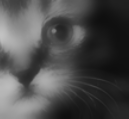
\includegraphics[width=3.5cm]{output_image_python/cat_part_ds10_rs100.png}
  }
  \quad
  \subfigure[$\sigma_d=10, \sigma_r=300$]{
  
\includegraphics[width=3.5cm]{output_image_python/cat_part_ds10_rs300.png}
  }
  \caption{A detail figure with bilateral filters with various range and domain parameter values by Opencv python}
  \label{py_cateye}
  \end{figure}
Fig.~\ref{py_cateye} indicates that the similarity of output between our re-implement code and the build-in algorithm in python, in other ways prove the successful implement of our code. the output looks very similar.

\begin{figure}[H]
  \centering
  \subfigure[$\sigma_d=1, \sigma_r=10$]{
  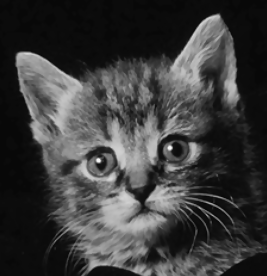
\includegraphics[width=3.5cm]{output_image/cat_ds1_rs10.png}
  % \caption{fig1}
  }
  \quad
  \subfigure[$\sigma_d=1, \sigma_r=30$]{
  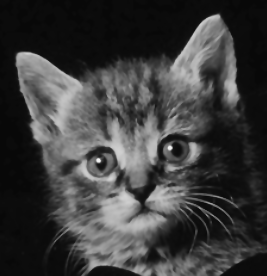
\includegraphics[width=3.5cm]{output_image/cat_ds1_rs30.png}
  }
  \quad
  \subfigure[$\sigma_d=1, \sigma_r=100$]{
  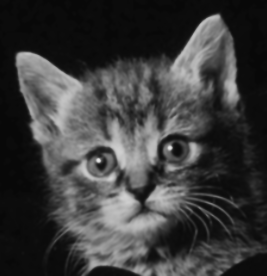
\includegraphics[width=3.5cm]{output_image/cat_ds1_rs100.png}
  }
  \quad
  \subfigure[$\sigma_d=1, \sigma_r=300$]{
  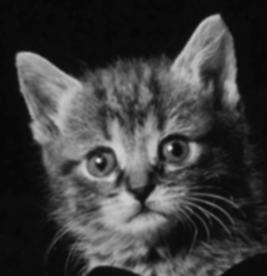
\includegraphics[width=3.5cm]{output_image/cat_ds1_rs300.png}
  }

  \subfigure[$\sigma_d=3, \sigma_r=10$]{
  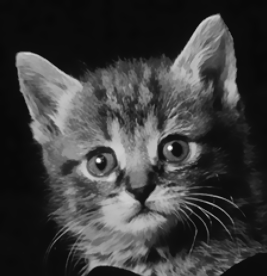
\includegraphics[width=3.5cm]{output_image/cat_ds3_rs10.png}
  % \caption{fig1}
  }
  \quad
  \subfigure[$\sigma_d=3, \sigma_r=30$]{
  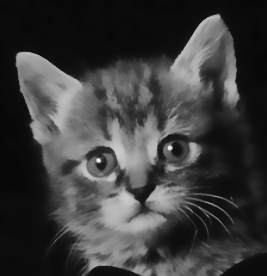
\includegraphics[width=3.5cm]{output_image/cat_ds3_rs30.png}
  }
  \quad
  \subfigure[$\sigma_d=3, \sigma_r=100$]{
  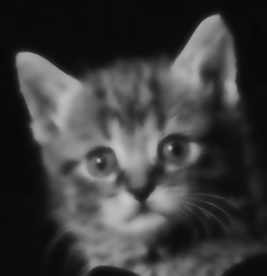
\includegraphics[width=3.5cm]{output_image/cat_ds3_rs100.png}
  }
  \quad
  \subfigure[$\sigma_d=3, \sigma_r=300$]{
  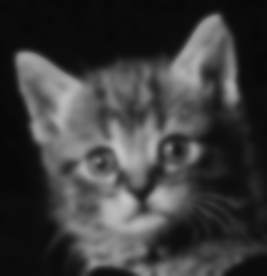
\includegraphics[width=3.5cm]{output_image/cat_ds3_rs300.png}
  }

  \subfigure[$\sigma_d=10, \sigma_r=10$]{
  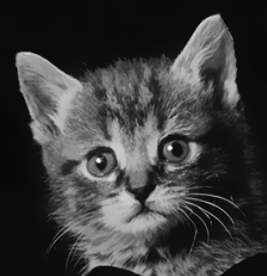
\includegraphics[width=3.5cm]{output_image/cat_ds10_rs10.png}
  % \caption{fig1}
  }
  \quad
  \subfigure[$\sigma_d=10, \sigma_r=30$]{
  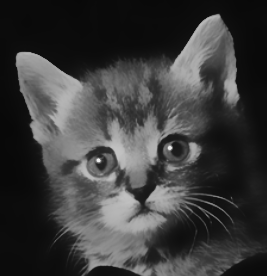
\includegraphics[width=3.5cm]{output_image/cat_ds10_rs30.png}
  }
  \quad
  \subfigure[$\sigma_d=10, \sigma_r=100$]{
  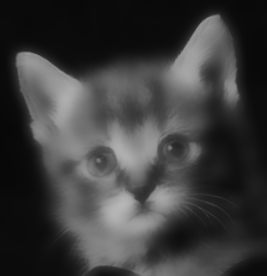
\includegraphics[width=3.5cm]{output_image/cat_ds10_rs100.png}
  }
  \quad
  \subfigure[$\sigma_d=10, \sigma_r=300$]{
  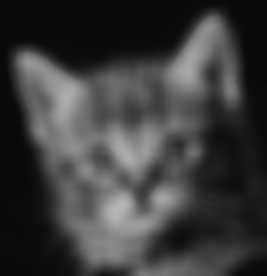
\includegraphics[width=3.5cm]{output_image/cat_ds10_rs300.png}
  }
  \caption{A detail figure with bilateral filters with various range and domain parameter values by re-implement code of cat}
  \label{im_cat}
  \end{figure}

\begin{figure}[H]
  \centering
  \subfigure[$\sigma_d=1, \sigma_r=10$]{
  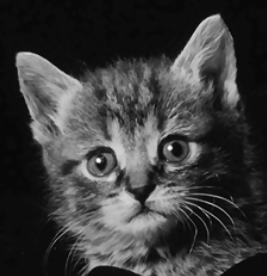
\includegraphics[width=3.5cm]{output_image_python/cat_ds1_rs10.png}
  % \caption{fig1}
  }
  \quad
  \subfigure[$\sigma_d=1, \sigma_r=30$]{
  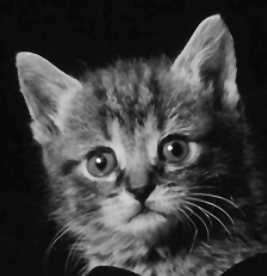
\includegraphics[width=3.5cm]{output_image_python/cat_ds1_rs30.png}
  }
  \quad
  \subfigure[$\sigma_d=1, \sigma_r=100$]{
  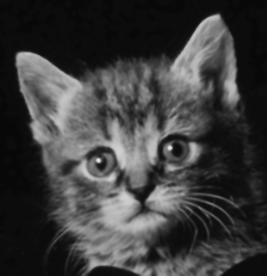
\includegraphics[width=3.5cm]{output_image_python/cat_ds1_rs100.png}
  }
  \quad
  \subfigure[$\sigma_d=1, \sigma_r=300$]{
  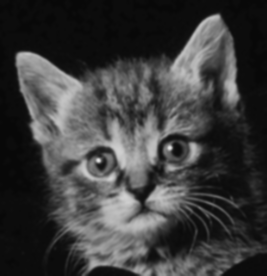
\includegraphics[width=3.5cm]{output_image_python/cat_ds1_rs300.png}
  }

  \subfigure[$\sigma_d=3, \sigma_r=10$]{
  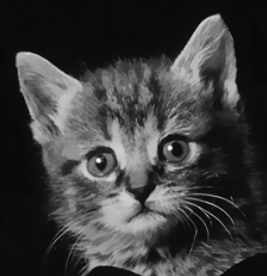
\includegraphics[width=3.5cm]{output_image_python/cat_ds3_rs10.png}
  % \caption{fig1}
  }
  \quad
  \subfigure[$\sigma_d=3, \sigma_r=30$]{
  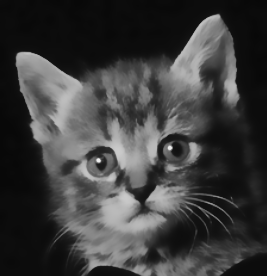
\includegraphics[width=3.5cm]{output_image_python/cat_ds3_rs30.png}
  }
  \quad
  \subfigure[$\sigma_d=3, \sigma_r=100$]{
  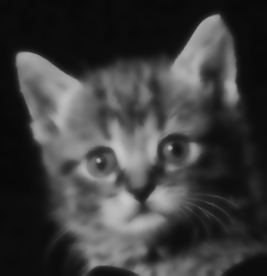
\includegraphics[width=3.5cm]{output_image_python/cat_ds3_rs100.png}
  }
  \quad
  \subfigure[$\sigma_d=3, \sigma_r=300$]{
  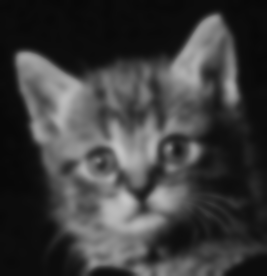
\includegraphics[width=3.5cm]{output_image_python/cat_ds3_rs300.png}
  }

  \subfigure[$\sigma_d=10, \sigma_r=10$]{
  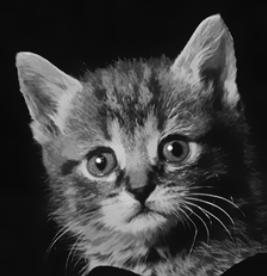
\includegraphics[width=3.5cm]{output_image_python/cat_ds10_rs10.png}
  % \caption{fig1}
  }
  \quad
  \subfigure[$\sigma_d=10, \sigma_r=30$]{
  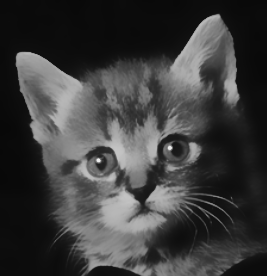
\includegraphics[width=3.5cm]{output_image_python/cat_ds10_rs30.png}
  }
  \quad
  \subfigure[$\sigma_d=10, \sigma_r=100$]{
  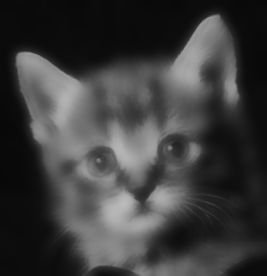
\includegraphics[width=3.5cm]{output_image_python/cat_ds10_rs100.png}
  }
  \quad
  \subfigure[$\sigma_d=10, \sigma_r=300$]{
  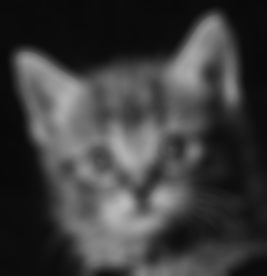
\includegraphics[width=3.5cm]{output_image_python/cat_ds10_rs300.png}
  }
  \caption{A detail figure with bilateral filters with various range and domain parameter values by Opencv python of cat}
  \label{py_cat}
  \end{figure}

Fig.~\ref{im_cat} and~\ref{py_cat} are also two image which prove the success of our re-implement code. 
In Fig.~\ref{table}, we also present another images that presented on the paper. 
As it presents, the salt and pepper noise can be removed, and also the edge information can be keeped as shown in Fig.~\ref{table_smmoth_onion} 


% The result indicates that our re-implement method of Bilateral filter can output the same grey result no matter compared with built-in opencv method or printed on paper.

\begin{figure}[H]
  \centering

  \subfigure[$\sigma_d=1, \sigma_r=10$]{
  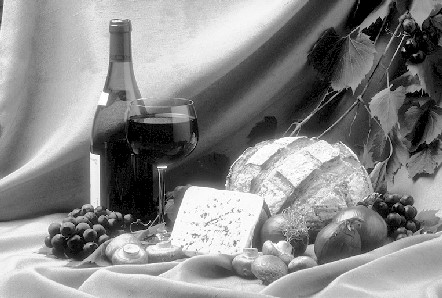
\includegraphics[width=7cm]{original_paper_images/snack.png}
  % \caption{fig1}
  }
  \quad
  \subfigure[$\sigma_d=1, \sigma_r=30$]{
  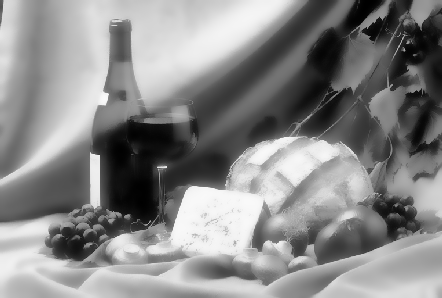
\includegraphics[width=7cm]{output_image/snack_ds3_rs50.png}
  }
  \quad
  \subfigure[$\sigma_d=1, \sigma_r=100$]{
  \includegraphics[width=7cm]{original_paper_images/onion.png}
  }
  \quad
  \subfigure[$\sigma_d=1, \sigma_r=300$]{
  \includegraphics[width=7cm]{output_image/onion_ds3_rs50.png}
  \label{table_smooth_onion}
  }
  \caption{A detail figure with bilateral filters with various range and domain parameter values by Opencv python of cat}
  \label{table}
\end{figure}

These images above indicate some other experiments which utilized the images provided by the paper.

There are some other color (3-channels) images which also indicate the successful re-implement of our code for bilateral filters.

\begin{figure}[H]
  \centering

  \subfigure[$\sigma_d=1, \sigma_r=10$]{
  \includegraphics[width=7cm]{original_paper_images/child.png}
  % \caption{fig1}
  }
  \quad
  \subfigure[$\sigma_d=1, \sigma_r=30$]{
  \includegraphics[width=7cm]{output_color_image/child_ds3_rs10.png}
  }
  \quad
  \subfigure[$\sigma_d=1, \sigma_r=100$]{
  \includegraphics[width=7cm]{original_paper_images/rubiks_cube.png}
  }
  \quad
  \subfigure[$\sigma_d=1, \sigma_r=300$]{
  \includegraphics[width=7cm]{output_color_image/rubiks_cube_ds3_rs50.png}
  }
  \quad
  \subfigure[sky]{
  \includegraphics[width=7cm]{original_paper_images/sky.png}
  }
  \quad
  \subfigure[sky code]{
  \includegraphics[width=7cm]{output_color_image/sky_ds3_rs30.png}
  }
  \quad
  \subfigure[home]{
  \includegraphics[width=7cm]{original_paper_images/home.png}
  }
  \quad
  \subfigure[home code]{
  \includegraphics[width=7cm]{output_color_image/home_ds3_rs30.png}
  }
  \caption{Color images filtered by Bilateral filter}
\end{figure}


\subsection{Compare with other baseline algorithm}
% in this section, compared with other blur algorithm
In this section, we compared the filter result of Bilateral filter with other baseline algorithm to present the advantages of our code.
In this experiment, we not only compared the output result passed by different filters from human version level, but also calculate the PNSR[cite paper] from mathmatical level. 
The equation of PNSR has been shwo in Equation:


\begin{figure}[H]
  \centering

  \subfigure[mean]{
  \includegraphics[width=7cm]{output_baseline/cat_mean_25.png}
  % \caption{fig1}
  }
  \quad
  \subfigure[median]{
  \includegraphics[width=7cm]{output_baseline/cat_median_25.png}
  }
  \quad
  \subfigure[gaussian]{
  \includegraphics[width=7cm]{output_baseline/cat_gaussian_25.png}
  }
  \quad
  \subfigure[Bilateral filter output]{
  \includegraphics[width=7cm]{output_image/cat_ds10_rs10.png}
  }
  \caption{output compared with the baseline low pass filters}
\end{figure}

The result indicates that the Bilateral filter has advantages compared with other low pass filter such as median filter, mean filter and gaussian filter.


% \begin{tabular}{cccccc}
%   \toprule  
%   Method& kernel\_size& $\sigma_d$& $\sigma_s$& PSNR\\
%   \midrule 
%   Bilateral Filter& 25& 1& 10 & 42.74\\
%                   &   &  & 30 & 32.26\\
%                   &   &  & 100& 32.59\\
%                   &   &  & 300& 31.70\\
%   \midrule
%   Bilateral Filter& 25& 3& 10 & 40.05\\
%                   &   &  & 30 & 31.37\\
%                   &   &  & 100& 25.90\\
%                   &   &  & 300& 24.39\\
%   \midrule
%   Bilateral Filter& 25& 10& 10 & 39.62\\
%                   &   &   & 30 & 29.72\\
%                   &   &   & 100& 22.38\\
%                   &   &   & 300& 20.31\\
%   \midrule
%   Median filter & 25& None & None & 20.31\\
%   Mean filter & 25 & None & None& 19.59\\
%   Gaussian filter& 25& None& None& 31.59\\
%   \bottomrule %添加表格底部粗线
%   \caption{The result of PSNR of difference method}
%   \label{}
% \end{tabular}
\begin{table}[]
\begin{tabular}{lllll}
\cline{1-5}
Method & Kernel\_size & sigma\_s & Sigma\_r & PSNR  \\ \cline{1-1}
\cline{1-5}
\multirow{4}{*}{Bilateral Filter}   & \multirow{4}{*}{25} & \multirow{4}{*}    {1}                               & 10      & 42.74 \\
       &             &            & 30      & 32.26     \\
       &             &            & 100     & 32.59     \\
       &             &            & 300     & 31.70     \\
\cline{1-5}
\multirow{4}{*}{Bilateral Filter}   & \multirow{4}{*}{25} & \multirow{4}{*}{3}  & 10       &40.05     \\
      &              &            & 30       & 31.37     \\
      &              &            & 100      & 25.90     \\
      &              &            & 300      & 24.39     \\
\cline{1-5}                                 
\multirow{4}{*}{Bilateral Filteral} & \multirow{4}{*}{25} & \multirow{4}{*}{10} & 10       & 39.62     \\
     &               &            & 30       & 29.72     \\
     &               &            & 100      & 22.38     \\
     &               &            & 300      & 20.31     \\
\cline{1-5}
Median filter       & 25          & None    & None     & 20.31     \\
Mean filter         & 25          & None    & None     & 19.59     \\
Gaussian filter          & 25           & None    & None     & 31.59    
\end{tabular}
\caption{The PSNR output of bailteral filter and baseline filters}
\label{table_PSNR}
\end{table}
The Tabel.~\ref{table_PSNR} presents the PSNR reult compared with Bilater filter and other baseline filters.

In the experiment, we use $kernel\_size = 25$ for all filters, but the same parameters as before in the paper. 
The result shows that the bilateral filter has advantages compared with other baseline low-pass filter. 
Only the Gaussian filter obtains $PSNR = 31.59$ which is very close with some result of the bilater filter and over some bery blur bilateral filters.
But still not good as the result with some very clean Bilater filters.

\end{document}
